\subsection{XHTML e XSL}
	\subsubsection {Falsi positivi}
\subsection{CSS}

\subsection{XML e XSD}
La validazione dei file XML rispetto agli schemi corrispondenti \`e stata effettuata tramite il seguente validatore on-line:
\\
\href{http://www.freeformatter.com/xml-validator-xsd.html}{http://www.freeformatter.com/xml-validator-xsd.html}
\begin{figure}[htbp]
	\centering
	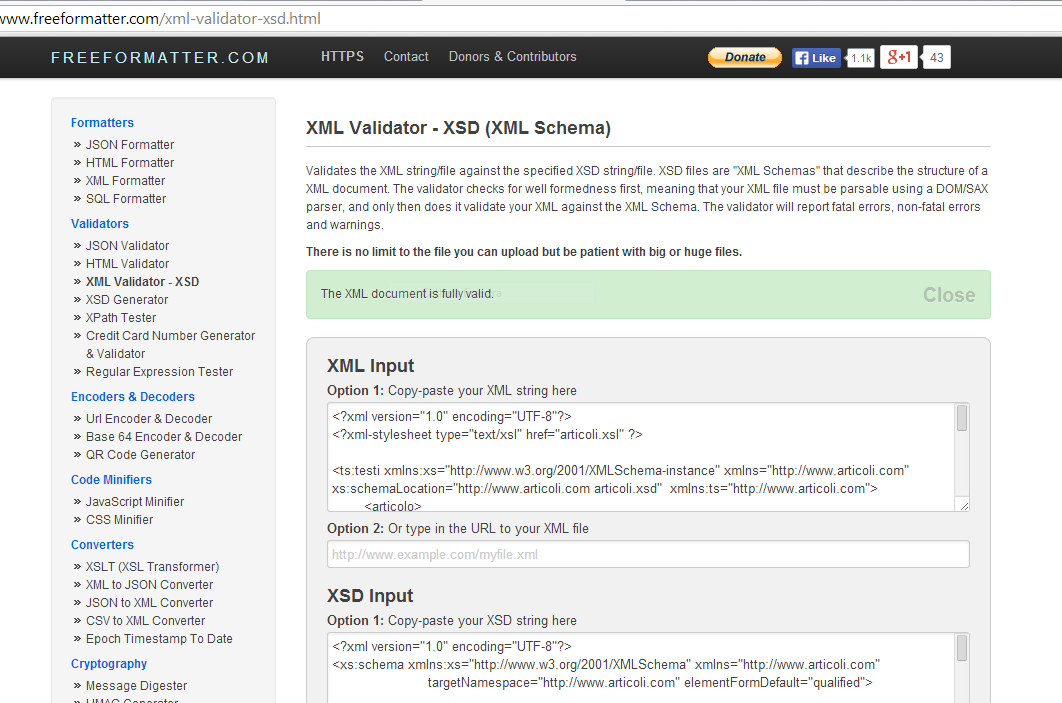
\includegraphics[width=105mm, height=13mm]{images/validazioneArticoli.png}
\end{figure}
Non è stato utilizzato il validatore del W3C poich\`e al momento non era funzionante.
